%&latex
%
\providecommand{\main}{../..}
\documentclass[../../main.tex]{subfiles}

\begin{document}

\section{Dynamics of the Ising Model}\label{sec:dynamics-ising}
\lesson{29}{14/05/20}

We are now ready to study the dynamics of the Ising Model. 

Each state $\bm{\sigma} = (\sigma_1, \dots, \sigma_N)$ is the spin configuration of all $N$ spins, with an associated energy given by:
\begin{align*}
    -\beta H(\bm{\sigma}) = K \sum_{\langle x,y \rangle} \sigma_x \sigma_y + h \sum_x \sigma_x
\end{align*}
As the spins are \textbf{binary} variables, the transition rate from a state $\bm{\sigma}$ to any configuration $\bm{\sigma'}$ can be written as a sum of \textit{spin-flip} rates:
\begin{align*}
    W(\bm{\sigma}'|\bm{\sigma}) = \sum_{x\>\mathrm{flips}} W_x(\bm{\sigma'}|\bm{\sigma})
\end{align*}  
For example, if $N=3$ and we consider tre transition $\bm{\sigma_1} \to \bm{\sigma_2}$ with:
\begin{align*}
    \bm{\sigma_1} = (+1,+1,+1) \qquad \bm{\sigma_2} = (\textcolor{Red}{-1},\textcolor{Red}{-1},+1)
\end{align*}
Then the transition rate is a sum of two spin-flip terms:
\begin{align*}
    W(\bm{\sigma_2}|\bm{\sigma_1}) = W_2[(+1,\textcolor{Red}{-1},+1)|(+1,+1,+1)] + W_3[(+1,+1,\textcolor{Red}{-1})|(+1,+1,+1)]
\end{align*}
Formally, $W_x(\bm{\sigma'}|\bm{\sigma})$ is the rate of the transition that flips the $x$-th spin in the $\bm{\sigma}$ configuration. If we define it in the following form:
\begin{align}\label{eqn:spin-flip-rate}
    W_x(\bm{\sigma'}|\bm{\sigma}) \propto \Big[\prod_{y \neq x} \delta_{\sigma_y, \sigma_{y'}}\Big] \delta_{\sigma_x, -\sigma_x'}
\end{align}
then it is automatically $0$ when the spin-flip is not needed (i.e. if $\sigma_x = \sigma_x'$), and so we can write:
\begin{align*}
    W(\bm{\sigma'}|\bm{\sigma}) = \sum_x W_x(\bm{\sigma'}|\bm{\sigma})
\end{align*}
with the sum extended over \textit{all} $N$ spins.

\medskip

We definitely know that the Ising Model has an \textbf{equilibrium state} - which was characterized in the previous chapters. So, we want the $W_x(\bm{\sigma}|\bm{\sigma'})$ to satisfy the detailed balance condition (\ref{eqn:detailed-balance}):
\begin{align}\label{eqn:db-flips}
    W_x(\bm{\sigma}|\bm{\sigma'}) e^{-\beta H(\bm{\sigma'})} = W_x(\bm{\sigma'}|\bm{\sigma}) e^{-\beta H(\bm{\sigma})}
\end{align}
As we are considering a single spin-flip transition at position $x$ (\ref{eqn:spin-flip-rate}), $H(\bm{\sigma'})$ differs from $H(\bm{\sigma})$ only for the different value of $\sigma_x$, and its interactions with the neighbouring spins $y \in \langle x,y \rangle$:
\begin{align*}
    -\beta H(\bm{\sigma'}) = -\beta H(\bm{\sigma}) - 2K \sigma_x \sum_{\mathclap{y \in \langle x,y \rangle}} \sigma_y - 2h \sigma_x
\end{align*}
Substituting in (\ref{eqn:db-flips}) and rearranging leads to:
\begin{align} \nonumber
    W_x(\bm{\sigma}|\bm{\sigma'}) \exp({\cancel{-\beta H(\bm{\sigma}) }- 2 K \sigma_x} \sum_{\mathclap{y \in \langle x,y \rangle}}\sigma_y - 2 h \sigma_x) = W_x(\bm{\sigma'}|\bm{\sigma}) \cancel{e^{-\beta H(\bm{\sigma})}} \span \\ \nonumber
    \Rightarrow \frac{W_x(\bm{\sigma'}|\bm{\sigma})}{W_x(\bm{\sigma}|\bm{\sigma'})} &= \exp\left(-2 K \sigma_x \sum_{\mathclap{y \in \langle x,y \rangle}}\sigma_y - 2 h \sigma_x\right) 
    = \frac{\displaystyle \exp\left(-\Big[ K \sum_{\mathclap{y \in \langle x,y \rangle}} \sigma_y + h \Big] \sigma_x \right)}{\displaystyle \exp\Bigg(\underbrace{\Big[ K \sum_{\mathclap{y \in \langle x,y \rangle}} \sigma_y + h\Big] }_{\mathtt{H}_x}\sigma_x\Bigg)} = \\
    &\underset{\mathclap{\substack{(\ref{eqn:ehsigma})\\\text{pag.} \pageref{eqn:ehsigma}}}}{=}\>\,  \frac{\bcancel{\cosh \mathtt{H}_x }(1 - \sigma_x \tanh \mathtt{H}_x)}{\bcancel{\cosh \mathtt{H}_x }(1+ \sigma_x \tanh \mathtt{H}_x)} = \frac{1-\sigma_x \tanh \mathtt{H}_x}{1 + \sigma_x \tanh \mathtt{H}_x} \label{eqn:transition-rate-db}
\end{align}
We can then choose any form for $W_x(\bm{\sigma'}|\bm{\sigma})$ that satisfies (\ref{eqn:transition-rate-db}) and it will lead at the end to the same equilibrium state. The simplest possibility is to just equate both sides numerators and denominators:
\begin{align}\label{eqn:flip-tran-rate}
    W_x(\bm{\sigma'}|\bm{\sigma}) &= \textcolor{Blue}{\frac{1}{2 \tau_m} } \Big[\prod_{z \neq x} \delta_{\sigma_z, \sigma_z'} \Big] \delta_{\sigma_x', -\sigma_x}\overbrace{\left[1- \sigma_x \tanh(h + K \sum_{\mathclap{y \in \langle x,y \rangle}} \sigma_y) \right]}^{w_x(\sigma_x, \bm{\hat{\sigma}_x})}  \\ \nonumber
    W_x(\bm{\sigma}|\bm{\sigma'}) &=  \textcolor{Blue}{\frac{1}{2 \tau_m} } \Big[\prod_{z \neq x} \delta_{\sigma_z, \sigma_z'} \Big] \delta_{\sigma_x', -\sigma_x}\overbrace{\left[1+ \sigma_x \tanh(h + K \sum_{\mathclap{y \in \langle x,y \rangle}} \sigma_y) \right]}^{w_x(-\sigma_x, \bm{\hat{\sigma}_x})}  =\\ \nonumber
    &\underset{\mathclap{(a)}}{=} \frac{1}{2 \tau_m} \Big[\prod_{z \neq x} \delta_{\sigma_z, \sigma_z'} \Big] \delta_{\sigma_x', -\sigma_x}\left[1- \sigma_x' \tanh(h + K \sum_{\mathclap{y \in \langle x,y \rangle}} \sigma_y') \right] =
\end{align} 
The symmetric factor $1/2\tau_m$ (independent of spin configuration) is added to fix the dimensions of $W_x$, which must be of $\mathsf{T}^{-1}$ as it is a transition \textit{rate}. Finally, in (a) we used the Kronecker $\delta$\textit{s} to rewrite $\sigma_x \to - \sigma_x'$ and $\sigma_y \to \sigma_y'$ for $y \neq x$.

We denote with $\bm{\hat{\sigma}_x} = \{\sigma_y \colon y \neq x\}$ all spins that \textit{do not} change during the spin flip. Then flipping the $x$-th spin amounts to the transition $(\sigma_x, \bm{\hat{\sigma}_x}) \to (-\sigma_x, \bm{\hat{\sigma}_x})$, and we denote its rate with $w_x(\sigma_x, \bm{\hat{\sigma}_x})$. Similarly, the reverse transition, i.e. $(-\sigma_x, \bm{\hat{\sigma}_x}) \to (\sigma_x, \bm{\hat{\sigma}_x})$ is denoted by $w_x(-\sigma_x, \bm{\hat{\sigma}_x})$.

\medskip

We can then write the Master Equation\marginpar{\vspace{1em}Master Equation for the Ising Model} (\ref{eqn:MasterEquation}) as follows:
\begin{align}\label{eqn:ising-ME}
    \dot{\mathbb{P}}(\bm{\sigma},t) = \sum_x \left[w_x(-\sigma_x, \bm{\hat{\sigma}_x}) \mathbb{P}(-\sigma_x, \bm{\hat{\sigma}_x}; t) - w_x(\sigma_x, \bm{\hat{\sigma}_x}) \mathbb{P}(\sigma_x, \bm{\hat{\sigma}_x};t)\right]
\end{align}
Note that the positive term is the \textit{inward flux of probability}, i.e. the one that goes from $-\sigma_x$ to the current state $\sigma_x$ (maintaining $\bm{\hat{\sigma}_x}$ the same), while the negative term is the \textit{outward flux} from $\sigma_x$ to $-\sigma_x$.   

\medskip

We can now compute the evolution of the average magnetization $\langle \sigma_z \rangle_t$ of the $z$-th spin:
\begin{align}\nonumber
    \dv{t} \langle \sigma_z \rangle_t &= \sum_{\{\bm{\sigma}\}} \mathbb{P}(\bm{\sigma},t) \sigma_z \underset{(\ref{eqn:ising-ME})}{=}  \sum_x \sum_{\{\bm{\sigma}\}} [\sigma_z w_x(-\sigma_x, \bm{\hat{\sigma}_x}) \mathbb{P}(-\sigma_x, \bm{\hat{\sigma}_x}) - \sigma_z w_x(\sigma_x, \bm{\hat{\sigma}_x}) \mathbb{P}(\sigma_x, \bm{\hat{\sigma}_x})] =\\
    \shortintertext{We split the sum between the terms with $x \neq z$ and the one with $x = z$:} \nonumber
    &= \sum_{x \neq z} \sum_{\{\bm{\sigma}\}} [\sigma_z w_x(-\sigma_x, \bm{\hat{\sigma}_x}) \mathbb{P}(-\sigma_x, \bm{\hat{\sigma}_x}) - \sigma_x w_x(\sigma_x, \bm{\hat{\sigma}_x}) \mathbb{P}(\sigma_x, \bm{\hat{\sigma}_x})] + \\ \label{eqn:avg-magnetization-ising}
    &\quad \>\>\>\> + \sum_{\{\bm{\sigma}\}} [\sigma_z w_z(-\sigma_z, \bm{\hat{\sigma}_z}) \mathbb{P}(-\sigma_z, \bm{\hat{\sigma}_z}) - \sigma_z w_z(\sigma_z, \bm{\hat{\sigma}_z}) \mathbb{P}(\sigma_z, \bm{\hat{\sigma}_z})]
\end{align}
In the first sum, note that:
\begin{align*}
    \sum_{\{\bm{\sigma}\}} \sigma_x w_x(\textcolor{Red}{-\sigma_x}, \bm{\hat{\sigma}_x}) \mathbb{P}(\textcolor{Blue}{-\sigma_x}, \bm{\hat{\sigma}_x}) = \sum_{\{\bm{\sigma}\}} \sigma_z w_x(\textcolor{Red}{\sigma_x}, \bm{\hat{\sigma}_x}) \mathbb{P}(\textcolor{Blue}{\sigma_x}, \bm{\hat{\sigma}_x})
\end{align*}
since we are summing over all possible configuration $\bm{\sigma}$. In general, for any function of the spins $\bm{\sigma}$:
\begin{align*}
    \sum_{\{\bm{\sigma}\}} f(\sigma_x, \bm{\hat{\sigma}_x}) = \sum_{\{\bm{\sigma}\}} f(-\sigma_x, \bm{\hat{\sigma}_x}) \qquad \forall f
\end{align*}
In fact, changing the sign of $\sigma_x$ merely amounts to a \textit{reordering} of the addends.

\medskip

So, if we make this change in the first term of the first sum, we get a cancellation:
\begin{align}\label{eqn:sum-a}
    \sum_{x \neq z} \sum_{\{\bm{\sigma}\}} [\sigma_z w_x(\textcolor{Red}{\sigma_x}, \bm{\hat{\sigma}_x}) \mathbb{P}(\textcolor{Red}{\sigma_x}, \bm{\hat{\sigma}_x}) - \sigma_x w_x(\sigma_x, \bm{\hat{\sigma}_x}) \mathbb{P}(\sigma_x, \bm{\hat{\sigma}_x})] = 0
\end{align}

Doing the same trick in the second sum, however, does \textit{not} lead to a cancellation:
\begin{align} \nonumber
    \sum_{\{\bm{\sigma}\}} [\textcolor{Red}{-\sigma_z} w_z(\textcolor{Red}{\sigma_z}, \bm{\hat{\sigma}_z}) \mathbb{P}(\textcolor{Red}{\sigma_z}, \bm{\hat{\sigma}_z}) - \sigma_z w_z(\sigma_z, \bm{\hat{\sigma}_z}) \mathbb{P}(\sigma_z, \bm{\hat{\sigma}_z})] = \span \\
    = -2 \sum_{\{\bm{\sigma}\}} \sigma_z w_z(\sigma_z, \bm{\hat{\sigma}_z}) \mathbb{P}(\sigma_z, \bm{\hat{\sigma}_z}) = -2 \langle \sigma_z w_z(\sigma_z, \bm{\hat{\sigma}_z}) \rangle_t \span \label{eqn:sum-b}
\end{align}

Substituting (\ref{eqn:sum-a}) and (\ref{eqn:sum-b}) back in (\ref{eqn:avg-magnetization-ising}) leads to:
\begin{align} \nonumber
    \partial_t \langle \sigma_z \rangle_t &= -2 \langle \sigma_z w_z(\sigma_z, \bm{\hat{\sigma}_z}) \rangle_t =\\ \nonumber
    &\underset{\mathclap{(\ref{eqn:flip-tran-rate})}}{=}  -\frac{\cancel{2}}{\cancel{2} \tau_m} \langle \sigma_z \Big[1 - \sigma_z \tanh\Big(h + K \sum_{\mathclap{y \in \langle x,y \rangle}} \sigma_y \Big)\Big] \rangle\\
    \Rightarrow \tau_m \langle \sigma_z \rangle_t &= -\langle \sigma_z \rangle_t + \langle \underbrace{\sigma_x^2}_{1}  \tanh \Big(h + K \sum_{\mathclap{y \in \langle x,y \rangle}} \sigma_y\Big) \rangle_t \label{eqn:avg-mag-z}
\end{align}
The second term can be expanded, taking into account that $\sigma_y = \pm 1$ is a binary variable. For example, in $d=1$, the spin neighbouring $z$ are $z-1$ and $z+1$:
\begin{align*}
    \tanh\Big(h + K(\sigma_{z+1} + \sigma_{z-1})\Big)
\end{align*}
Since $\sigma_{z\pm 1} = \pm 1$, this function can assume only $3$ possible values: one when $\sigma_{z\pm1} = +1$, another when $\sigma_{z \pm 1} = -1$, and the third one when $\sigma_{z+1} = +1$ and $\sigma_{z-1} = -1$ (or viceversa). A second order polynomial can be used to \textit{fit} these three points:
\begin{align*}
    \tanh(h + K(\sigma_{z+1} + \sigma_{z-1})) \overset{!}{=}  \hat{a} + \hat{b} (\sigma_{z+1} + \sigma_{z-1}) + \hat{c} (\sigma_{z+1} + \sigma_{z-1})^2
\end{align*} 
By expanding the square, note that $\sigma_{z \pm 1}^2 \equiv 1$. So, changing the coefficients accordingly, we have:
\begin{align}\label{eqn:polynomial-expansion}
    \tanh(h + K(\sigma_{z+1} + \sigma_{z-1})) \overset{!}{=}  a + b(\sigma_{z+1} + \sigma_{z-1}) + c \sigma_{z+1} \sigma_{z-1}
\end{align}
To find $a$, $b$ and $c$, note that if we sum over $\sigma_{z\pm 1} = \pm 1$ we get:
\begin{align*}
    \sum_{\mathclap{\sigma_{z\pm1} = \pm 1}}\quad \Big[ a + b(\sigma_{z+1} + \sigma_{z-1}) + c \sigma_{z+1} \sigma_{z-1} \Big] = 4a + (2b -2b) + (2c - 2c) = 4a
\end{align*}
And so:
\begin{align*}
    4a \overset{!}{=} \sum_{\sigma_{z\pm 1} = \pm 1} \tanh(h + K(\sigma_{z+1} + \sigma_{z-1})) &= 2 \tanh h + \tanh (h + 2K) + \tanh(h - 2K) 
\end{align*}
Note that if $h=0$, the right side vanishes, and so $a=0$.

\medskip

For the $b$ term, we first multiply by $\sigma_{z+1}$ and then sum over all possibilities:
\begin{align*} 
    4b = \sum_{\mathclap{\sigma_{z\pm1} = \pm 1}} \quad \sigma_{z+1}\Big[ a + b(\sigma_{z+1} + \sigma_{z-1}) + c \sigma_{z+1} \sigma_{z-1} \Big] = \span\\
    = \sum_{\mathclap{\sigma_{z\pm1} = \pm 1}} \quad \sigma_{z+1}\tanh(h + K(\sigma_{z+1} + \sigma_{z-1})) = \tanh(h + 2K) - \tanh(h - 2K) \span
\end{align*}
And finally, for the $c$ term we first multiply by $\sigma_{z+1} \sigma_{z-1}$:
\begin{align*} 
    4c = \sum_{\mathclap{\sigma_{z\pm1} = \pm 1}} \quad \sigma_{z+1} \sigma_{z-1}\Big[ a + b(\sigma_{z+1} + \sigma_{z-1}) + c \sigma_{z+1} \sigma_{z-1} \Big] = \span\\
    = \sum_{\mathclap{\sigma_{z\pm1} = \pm 1}} \quad \sigma_{z+1} \sigma_{z-1}\tanh(h + K(\sigma_{z+1} + \sigma_{z-1})) = -2 \tanh h + \tanh (h + 2K) + \tanh (h-2K) \span
\end{align*}
And again, if $h=0$ then $c=0$.

\medskip

Substituting (\ref{eqn:polynomial-expansion}) back in (\ref{eqn:avg-mag-z}) we arrive to:
\begin{align}\label{eqn:magnetization-evolution}
    \tau_m \dv{t} \langle \sigma_z \rangle_t = -\langle \sigma_z \rangle_t + a+ b(\langle \sigma_{z+1} \rangle_t + \langle \sigma_{z-1} \rangle_t) + c \langle \sigma_{z+1} \sigma_{z-1} \rangle_t
\end{align}
which cannot be solved unless we know $\langle \sigma_{z+1} \sigma_{z-1} \rangle_t$. However, if we compute $\partial_t \langle \sigma_{z+1} \sigma_{z-1} \rangle$, the resulting expression will involve other correlations, leading to many coupled equations.

However, if $h=0$ we know that $a = c = 0$. This, at least in $d=1$ case, allows to write a closed-form solution of (\ref{eqn:magnetization-evolution}), which was found by Glauber in 1961. For $d > 1$, (\ref{eqn:magnetization-evolution}) contains also higher order correlations, that cannot be neglected when $h=0$, making the problem unsolvable in general.

\section{Mean Field Dynamics}
Solving the dynamics of the Ising Model is hard task already in $d=1$, and it is effectively intractable in $d > 1$. 

So, to proceed, we make use of the \textbf{mean field approximation}. We start from (\ref{eqn:avg-mag-z}):
\begin{align*}
    \tau_m \partial_t \underbrace{\langle \sigma_z \rangle_t}_{m_z(t)}  = - \langle \sigma_z \rangle_t + \langle \tanh \Big(h + K \sum_{\mathclap{y \in \langle x,y \rangle}} \sigma_y \Big)  \rangle_t
\end{align*}
and take the average \textbf{inside} the $\tanh$:
\begin{align}\label{eqn:mean-field-dynamics}
    \tau_m \partial_t m_z(t) = -m_z(t) + \tanh \Big(h + K \sum_{\mathclap{y \in \langle x,y \rangle}} m_y(t) \Big)
\end{align} 
In this way, we get a \textit{closed} equation for the magnetization!

\medskip

At stationarity (e.g. at equilibrium), $\partial_t m_z(t) \equiv 0$, meaning that $m_z(t) \equiv M_z$ is constant, and satisfies:
\begin{align*}
    M_z = \tanh \Big( h + K \sum_{\mathclap{y \in \langle x,y \rangle}} M_y\Big)
\end{align*}
which is exactly the equation we got by using the variational principle and the mean field approximation (\ref{eqn:variational-sol}, pag. \pageref{eqn:variational-sol}). 

\subsection{Uniform solution}

Returning to the full equation (\ref{eqn:mean-field-dynamics}), note that if we choose a \textbf{uniform} initial condition $m_z(t=0) \equiv m(t=0)$ independent of $z$, then the symmetry cannot be broken - as all spins evolve in the same way - and so $m_z(t) \equiv m(t)$ $\forall t > 0$, leading to:
\begin{align}\label{eqn:uniform-evolution}
    \tau_m \dot{m}(t) = -m(t) + \tanh(h + 2dKm(t))
\end{align} 
where $2d$ is the number of neighbours of any spin in a $d$-dimensional cubic lattice (with p.b.c.).

Equation (\ref{eqn:uniform-evolution}) can be solved numerically. To get some insight, we take $h=0$ and $m(0) \approx 0$ near the critical point $2dK \approx 1 \Rightarrow K \approx K_c = 1/2d$. Expanding the $\tanh$ in series:
\begin{align}\label{eqn:uniform-expansion}
    \tau_m \dot{m} &= -m + 2dK m - \frac{1}{3}(2dK)^3 m^3 + \dots = -k m - \eta m^3 + \dots \span
    \shortintertext{with:} \nonumber
    k = 1 - 2dK = 1 - \frac{K}{K_c} = \frac{K_c - K}{K_c}; \qquad \eta = \frac{1}{3} \frac{K}{K_c} \underset{K \approx K_c}{=}  \frac{1}{3} + O(k)   \span    
\end{align}

Let's see what happens in the various regimes $T > T_c$, $T=T_c$ and $T < T_c$:
\begin{itemize}
    \item $T > T_c \Leftrightarrow K < K_c \Rightarrow k > 0$. We then make a change of variables $m \to x$, with:
    \begin{align*}
        m(t) = \exp(-\frac{k t}{\tau_m}) x(t)
    \end{align*} 
    In this way, when substituting in (\ref{eqn:uniform-expansion}) we get a cancellation:
    \begin{align*}
        - \cancel{\frac{k \tau_m}{\tau_m} \exp\left(-\frac{kt}{\tau_m} \right)  x} + \tau_m \exp\left(-\frac{kt}{\tau_m} \right) \dot{x} = -\cancel{k \exp\left(-\frac{kt}{\tau_m} \right) x} - \eta x^3 \exp\left(-\frac{3kt}{\tau_m} \right) \span\\
        \Rightarrow \tau_m \dot{x}(t) = -\eta x(t)^3 \exp\left(-\frac{2kt}{\tau_m} \right) \span
    \end{align*}
    which can be solved by separation of variables:
    \begin{align*}
        \frac{\dd{x}}{x^3} = -\eta \exp\left(-\frac{2kt}{\tau_m} \right)  \frac{\dd{t}}{\tau_m}
    \end{align*}
    leading to:
    \begin{align*}
        m(t) = \sqrt{k} \left[\exp\left(\frac{2kt}{\tau_m} \right) \left(\frac{k}{m^2(0)} + \eta \right) - \eta\right]^{-1/2}\> \underset{\mathclap{t \gg \tau_m/k \equiv \tau_+}}{\sim}\>  \sqrt{k} \exp\left(-\frac{kt}{\tau_m} \right)
    \end{align*}
    When $t \to +\infty$, as $k > 0$, the exponential term diverges, meaning that the magnetization vanishes with a characteristic timescale $\tau_+$: 
    \begin{align}\label{eqn:characteristic-time-scaling}
        \tau_+ \equiv \tau_m k^{-1} = \left(\frac{T-T_c}{T_c} \right)^{-1}
    \end{align}
    which \textbf{diverges} when $T \to T_c^+$. This behaviour is similar to that of the correlation length $\xi(T)$:
    \begin{align}\label{eqn:corr-length-scaling2}
        \xi(T) \propto \left|\frac{T-T_c}{T_c}  \right|^{-1/2}
    \end{align}
    In fact, in general it can be shown that these tow scalings are related:
    \begin{align}\label{eqn:dynamical-exponent}
        \tau_+ = \xi^z
    \end{align}
    where $z$ is called the \textbf{dynamical exponent}. Comparing (\ref{eqn:characteristic-time-scaling}) to (\ref{eqn:corr-length-scaling2}) we see that, in the mean field approximation, $z = 2$.
    \item $T = T_c \Leftrightarrow K = K_c \Rightarrow k=0$. Equation (\ref{eqn:uniform-expansion}) becomes (neglecting higher order terms): 
    \begin{align*}
        \tau_m \dot{m} = - \eta m^3
    \end{align*}
    and can be immediately solved by separation of variables:
    \begin{align*}
        \frac{\dd{m}}{m^3} = - \eta \frac{\dd{t}}{\tau_m} \Rightarrow m(t) = \frac{m(0)}{\sqrt{1 + m^2(0) \eta t/\tau_m}} \quad \>\> \underset{\mathclap{t \gg \frac{\tau_m}{2m^2(0)\eta} }}{\sim} \quad \left(\frac{t}{\tau_m} \right)^{-\textcolor{Red}{\frac{1}{2}}}
    \end{align*}
    Note that while for $T > T_c$ we found that $m(t)$ decays exponentially, for $T=T_c$ it decays following a power law - i.e. much more slowly (see fig. \ref{fig:magnetization-evolution}). This is the so-called \textbf{critical slowing down}.  
    \item If $T < T_c$ ($K > K_c$ and $k < 0$), (\ref{eqn:uniform-expansion}) becomes:
    \begin{align*}
        \tau_m \dot{m} = |k| m - \eta m^3
    \end{align*}
    The \textbf{positive} linear term will make $m$ grow \textit{exponentially} at the start, and then stabilize to some value (depending on the initial condition) due to the \textbf{negative} cubic term.
    
    In fact, at stationarity $\dot{m} = 0$, and two solutions are possible: $m=0$ and $m = \sqrt{|k|/\eta} \equiv m_\infty$, which describes the \textit{spontaneous magnetization}. 
    
    Changing variables:
    \begin{align*}
        m(t) = \exp\left(\frac{|k|t}{\tau_m} \right) x(t)
    \end{align*}
    leads to: %TODO Missing steps
    \begin{align*}
        m(t) &= m_\infty \left[1 + \exp\left(-\frac{2|k|t}{\tau_m} \right) \left(\frac{m^2_\infty}{m^2(0)} - 1 \right)\right]^{-\frac{1}{2}} \\
        &\underset{\mathclap{t \gg \tau_m/|k|}}{\sim} \quad m_\infty \left[1-\frac{1}{2} \exp\left(-\frac{2|k|t}{\tau_m} \right)\left(\frac{m^2_\infty}{m^2(0)} -1\right) \right]
    \end{align*}
    Again we find an \textit{emerging} characteristic timescale:
    \begin{align*}
        \tau_- \equiv \frac{\tau_m}{2|k|} = \frac{\tau_m}{2} \left|\frac{T-T_c}{T_c}  \right|^{-1} \propto \xi^z \qquad z=2
    \end{align*} 
    
    Thus $\tau_\pm \propto \xi^z$ for both $T > T_c$ and $T < T_c$. 
\end{itemize}

\begin{figure}[H]
    \centering
    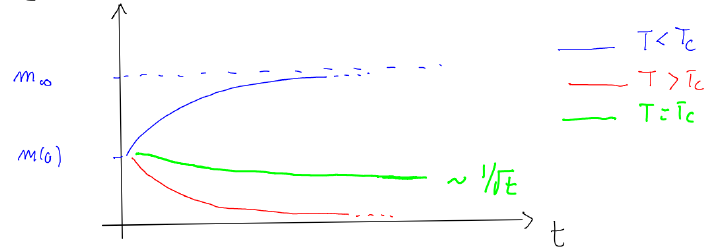
\includegraphics[width=0.9\textwidth]{\main/Images/magnetization-evolution.png}
    \caption{The evolution of the magnetization $m(t)$ in the mean field approximation with a uniform starting condition and near criticality.}
    \label{fig:magnetization-evolution}
\end{figure}

\subsection{Non-uniform case}
Let's return to (\ref{eqn:mean-field-dynamics}), this time assuming a magnetization that is \textit{everywhere \q{small}}, but non-uniform.

Let $h=0$ and $t > T_c$ (high temperature phase). If we expand the $\tanh$ in series:
\begin{align*}
    \tanh \Big(K \sum_{\mathclap{y \in \langle x,y \rangle}} m_y\Big) = K \sum_{\mathclap{y \in \langle x,y \rangle}} m_y + O(m^3)
\end{align*}
equation (\ref{eqn:mean-field-dynamics}) becomes:
\begin{align}\nonumber
    \tau_m \dot{m}_x &= - m_x + K \sum_{\mathclap{y \in \langle x,y \rangle}} m_y + \dots =\\
    &= -m_x + K \sum_{\mu=1}^d (m_{\bm{r}_x + a \bm{\hat{\mu}}} + m_{\bm{r}_x - a \bm{\hat{\mu}}}) \label{eqn:non-uniform-evolution}
\end{align}
where $\bm{r}_x$ is the position of the $x$-th spin, and $\bm{\hat{\mu}}$ is a unit vector pointing along the $d$-th dimension. For every direction $d$, the two neighbour of $x$ are at positions $\bm{r}_x \pm a \bm{\hat{\mu}}$ in the cubic lattice.

\medskip

Since we are near criticality, we expect the magnetization to change \textit{smoothly} in space\footnote{Or, in other words, the \textit{correlation length} $\xi$ is much higher than the lattice spacing $a$}, justifying the following expansion:
\begin{align}\label{eqn:magnetization-expansion}
    m_{\bm{r}_x \pm a \bm{\hat{\mu}}} = m_x \pm a \partial_\mu m_x + \frac{a^2}{2} \partial_\mu^2 m_x + \dots  
\end{align} 
Then the sum in (\ref{eqn:non-uniform-evolution}) becomes:
\begin{align*}
    \sum_{\mu=1}^d (m_{\bm{r}_x + a\bm{\hat{\mu}}} + m_{\bm{r}_x - a \bm{\hat{\mu}}}) = 2d m_x + \frac{a^2}{2} \nabla^2 m_x + \dots 
\end{align*}
and the full equation is:
\begin{align*}
    \tau_m \dot{m}_x = \underbrace{(2dK - 1)}_{\mathclap{\frac{K - K_c}{K_c} = -k; \quad k > 0}} m_x + \frac{a^2}{2} K \nabla^2 m_x 
\end{align*}
Dividing by $\tau_m$, the $\tau_+$ term defined in (\ref{eqn:characteristic-time-scaling}) reappears:
\begin{align}\label{eqn:magnetization-diffusion}
    \dot{m}_x = \hlc{Yellow}{- \frac{1}{\tau_+} m_x }+ D \nabla^2 m_x \qquad D \equiv \frac{a^2 k}{2 \tau_m}; \> \tau_+ \equiv \frac{\tau_m}{k} 
\end{align}
which looks like the diffusion equation, with a diffusion constant $D$ of dimensions $\mathsf{L}^2\mathsf{T}^{-1}$.

If the highlighted term were $0$, then the magnetization would be \q{conserved}, in the sense that the integral of $m_x$ over $x$ is constant in time.

\medskip

Equation (\ref{eqn:magnetization-diffusion}) can be solved by using a Fourier transform:
\begin{align*}
    m_{\bm{r}_x}(t) = \int_{\mathbb{R}^d} \tilde{m}_{\bm{q}}(t) e^{i \bm{q} \cdot \bm{r}_x} \frac{\dd[d]{\bm{q}}}{(2\pi)^d} \qquad \tilde{m}_{\bm{q}} = \int_{\mathbb{R}^d} e^{-i \bm{q} \cdot \bm{r}_x} m_{\bm{r}_x} \dd[d]{\bm{r}_x}
\end{align*}
Differentiating with respect to $t$:
\begin{align}\label{eqn:non-uniform-transformed}
    \partial_t \tilde{m}_{\bm{q}}(t) \underset{(\ref{eqn:magnetization-diffusion})}{=}  -\left(\frac{1}{\tau_+} + D \norm{\bm{q}}^2\right) \tilde{m}_{\bm{q}}(t)
\end{align}
Note that all the coordinates of $\bm{q}$ are independent from each other, i.e. there isn't any mixed term $q_i q_j$ with $i \neq j$. On the other hand, this was not the case in (\ref{eqn:magnetization-diffusion}), as due to the laplacian, each $m_x$ had some dependence on the neighbouring spins.

\medskip

So, (\ref{eqn:non-uniform-transformed}) is much simpler than (\ref{eqn:magnetization-diffusion}), and in fact it can be solved by separation of variables, leading to:
\begin{align}\label{eqn:transformed-sol}
    \tilde{m}_{\bm{q}}(t) = \exp\left(-\left[\frac{1}{\tau_+} + D \norm{\bm{q}}^2 \right] t\right) \tilde{m}_{\bm{q}}(0)
\end{align}
where $\tilde{m}_{\bm{q}}(0)$ is the Fourier transform of the initial condition $m_{\bm{r}_x}(0)$:
\begin{align*}
    \tilde{m}_{\bm{q}}(0) = \int_{\bm{R}^d} \dd[d]{\bm{r}_y} e^{-i \bm{q} \cdot \bm{r}_y} m_{\bm{r}_y}(0)
\end{align*}

All that's left is to anti-transform (\ref{eqn:transformed-sol}):
\begin{align}\nonumber
    m_{\bm{r}_x}(t) &= \int_{\mathbb{R}^d} \left[ \int_{\mathbb{R}^d} \exp\left(-\left[\frac{1}{\tau_+} + D \norm{\bm{q}}^2 \right] t + i \bm{q} \cdot (\bm{r}_x - \bm{r}_y)\right) \frac{\dd[d]{\bm{q}}}{(2\pi)^d} \right] m_{\bm{r}_y}(0) \dd[d]{\bm{r}_y} =\\
    \shortintertext{which is a gaussian integral and evaluates to:} \label{eqn:non-uniform-sol}
    &= \frac{e^{-t/\tau_+}}{(4 \pi D t)^{d/2}} \int_{\mathbb{R}^d} \exp\left(-\frac{\norm{\bm{r}_x - \bm{r}_y}^2}{4 D t} \right) m_{\bm{r}_y}(0) \dd[d]{\bm{r}_y}
\end{align}

We were able to compute this solution only because $T > T_c$, meaning that we can neglect the $m^3$ term of the $\tanh$ expansion (\ref{eqn:uniform-expansion}). That non-linear term is important only for $T < T_c$, where it \textit{stops} the diverging growth of the now positive linear term. Also, we need to be \textit{close} to criticality ($T \to T_c^+$) in order to justify the expansion in (\ref{eqn:magnetization-expansion}). 

\begin{example}[Single magnetized spin]
    Consider the initial condition where only the spin at the origin has a $M \neq 0$ magneitzation:
    \begin{align*}
        m_{\bm{r}_y}(t=0) = M \delta^d(\bm{r}_y)
    \end{align*}
    Then (\ref{eqn:non-uniform-sol}) becomes:
    \begin{align*}
        m_{\bm{r}_x}(t) = \frac{e^{-t/\tau_+}}{(4 \pi D t)^{d(2)}} \exp\left(-\frac{\norm{\bm{r}_x}^2}{4 D t} \right) M
    \end{align*}
    Graphically, the magnetization \textit{decays} in time by \q{spreading} to the neighbouring spins in a \textit{gaussian} way (fig. \ref{fig:single-magnetized-evo}). 
    
    \medskip

    If we integrate over all positions, we find that the magnetization \textit{is not conserved}: 
    \begin{align}\label{eqn:magnetization-decay}
        \int_{\mathbb{R}^d} \dd[d]{\bm{r}_x} m_{\bm{r}_x}(t) = M e^{-t/\tau_+}
    \end{align}
    For $t \to +\infty$ we will have $m_{x} \equiv 0$ $\forall x$.

    \medskip

    It can be shown that (\ref{eqn:magnetization-decay}) is independent of the specific initial condition - meaning that for $T > T_c$, the magnetization will always decay.
\end{example}

\begin{figure}[H]
    \centering
    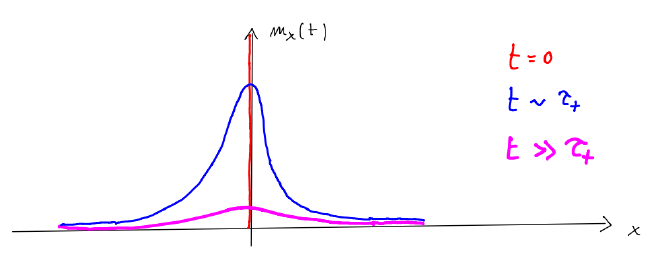
\includegraphics[width=0.8\textwidth]{\main/Images/single-magnetized-evo.png}
    \caption{Time evolution of the average magnetization in a $d=1$ system, with only the spin at the origin initially magnetized.}
    \label{fig:single-magnetized-evo}
\end{figure}

\begin{exo}[Evolution of a gaussian magnetization]
    Consider the following initial condition:
    \begin{align*}
        m_{\bm{r}_y}(t=0) = \frac{M}{(\sigma \sqrt{2 \pi})^d} \exp\left(-\frac{\norm{\bm{r}_y}^2}{2 \sigma^2} \right) \qquad \int_{\mathbb{R}^d} \dd[d]{\bm{r}_y} m_{\bm{r}_y}(0) = M
    \end{align*}
    Compute its evolution $m_{\bm{r}_x}(t)$ according to equation (\ref{eqn:non-uniform-sol}).

    \medskip

    \textbf{Solution}. 
\end{exo}

\begin{exo}[Magnetization's decay]
    Show that (\ref{eqn:magnetization-diffusion}) implies that:
    \begin{align*}
        M(t) \equiv \int_{\mathbb{R}^d} \dd[d]{\bm{r}_x} m_{\bm{r}_x}(t) = e^{-t/\tau_+} M(0)
    \end{align*}

    \medskip

    \textbf{Solution}. 
\end{exo}

\begin{exo}[Chemical reaction]
    Consider the chemical reaction $X\leftrightharpoons A$ where the number of $A$ is kept fixed at $a$. The reaction $X \leftarrow A$ occurs at a rate $k_2$ per particle of kind $A$ whereas the reaction $X \rightarrow A$ occurs at a rate $k_1$ per particle of kind $X$. Determine:
    \begin{enumerate}
        \item the transition rates $W(x \pm 1|x)$;
        \item the master equation for $\mathbb{P}(x,t)$, the probability that at time $t$ there are $x$ particles of kind $X$;
        \item the stationary state, $\mathbb{P}^*(x)$;
        \item the equation obeyed by $\dd{\langle f(x) \rangle}/\dd{t}$ for a generic function $f$;
        \item the time dependence of $\langle x \rangle$ and its infinite time limit;
        \item the equation obeyed by $\dd{G(s,t)}/\dd{t}$ where:
        \begin{align*}
            G(s,t) = \sum_{x \geq 0} s^x \mathbb{P}(x,t)
        \end{align*}
        is the generating function;
        \item the solution of $G(s,t)$ if the initial condition is $\mathbb{P}(x,t=0) = \delta_{x,N}$;
        \item the solution of $\mathbb{P}(x,t)$ if $N=0$
    \end{enumerate}
    
\end{exo}


\end{document}
